\documentclass[11pt]{cernrep}
\usepackage{graphicx,epsfig}
\bibliographystyle{lesHouches}

\usepackage{xspace}
\newcommand{\Sherpa}{S\protect\scalebox{0.8}{HERPA}\xspace}
\newcommand{\Powheg}{P\protect\scalebox{0.8}{OWHEG}\xspace}
\newcommand{\CSS}{C\protect\scalebox{0.8}{SS}\xspace}
\newcommand{\Comix}{C\protect\scalebox{0.8}{OMIX}\xspace}
\newcommand{\Amegic}{A\protect\scalebox{0.8}{MEGIC++}\xspace}
\newcommand{\MCatNLO}{M\protect\scalebox{0.8}{C}@N\protect\scalebox{0.8}{LO}\xspace}
\newcommand{\MEPS}{M\scalebox{0.8}{E}P\scalebox{0.8}{S}\xspace}
\newcommand{\MEPSatNLO}{M\scalebox{0.8}{E}P\scalebox{0.8}{S}@N\protect\scalebox{0.8}{LO}\xspace}
\newcommand{\Collier}{C\protect\scalebox{0.8}{OLLIER}\xspace}
\newcommand{\OpenLoops}{O\protect\scalebox{0.8}{PEN}L\protect\scalebox{0.8}{OOPS}\xspace}
\newcommand{\Herwig}{H\protect\scalebox{0.8}{ERWIG}7\xspace}
\newcommand{\Matchbox}{M\protect\scalebox{0.8}{ATCHBOX}\xspace}
\newcommand{\MGaMC}{M\protect\scalebox{0.8}{AD}G\protect\scalebox{0.8}{RAPH}5\_aMC@NLO\xspace}
\newcommand{\MadGraph}{M\protect\scalebox{0.8}{AD}G\protect\scalebox{0.8}{RAPH}\xspace}
\newcommand{\MadGraphfour}{M\protect\scalebox{0.8}{AD}G\protect\scalebox{0.8}{RAPH}4\xspace}
\newcommand{\CVolver}{CV\protect\scalebox{0.8}{OLVER}\xspace}
\newcommand{\ColorFull}{C\protect\scalebox{0.8}{OLOR}F\protect\scalebox{0.8}{ULL}\xspace}
\newcommand{\pt}{\ensuremath{p_{T}}\xspace}
\newcommand\sss{\mathchoice%
{\displaystyle}%
{\scriptstyle}%
{\scriptscriptstyle}%
{\scriptscriptstyle}%
}
\newcommand\MSB{\ifmmode {\overline{\rm MS}} \else $\overline{\rm MS}$\fi}
\newcommand\MINLO{{\tt MiNLO}}
\newcommand\muf{\mu_{\sss\rm F}}
\newcommand\mur{\mu_{\sss\rm R}}
\newcommand\KRA{K_{\scriptscriptstyle \rm R}}
\newcommand\KFA{K_{\scriptscriptstyle \rm F}}

\newcommand{\GOSAM}{G\protect\scalebox{0.8}{O}S\protect\scalebox{0.8}{AM}\xspace}
\newcommand{\POWHEGBOX}{P\protect\scalebox{0.8}{OWHEG} B\protect\scalebox{0.8}{OX}\xspace}
\newcommand{\QGRAF}{Q\protect\scalebox{0.8}{GRAF}\xspace}
\newcommand{\FORM}{F\protect\scalebox{0.8}{ORM}\xspace}
\newcommand{\SAMURAI}{S\protect\scalebox{0.8}{AMURAI}\xspace}
\newcommand{\GOLEM}{G\protect\scalebox{0.8}{OLEM}\xspace}
\newcommand{\NINJA}{N\protect\scalebox{0.8}{INJA}\xspace}
\newcommand{\SPINNEY}{S\protect\scalebox{0.8}{PINNEY}\xspace}
\newcommand{\ONELOOP}{O\protect\scalebox{0.8}{NE}LO\protect\scalebox{0.8}{OP}\xspace}
\newcommand{\MCFM}{M\protect\scalebox{0.8}{CFM}\xspace}


\usepackage{color}
\usepackage{morefloats}

\begin{document}

\section{Study of electroweak production of WZ in association with two
  jets at the LHC \protect\footnote{Section
    coordinators:K.~D.~Long, M.~Pellen}$^{,}$ \protect\footnote{Contributing authors:
    S.~Br\"auer, V.~Ciulli, M.~Herndon, S.~Gieseke, S.~Platzer,
    M.~Rauch, E.~Yazgan,...}$^{,}$
  \protect\footnote{{\it next some examples of aknwoledgments}}$^{,}$
  \protect\footnote{ A. Aaaaa acknowledges support by a FP7 Marie
    Curie Intra European Fellowship under Grant Agreement xxxx.}$^{,}$
\protect\footnote{The work of B. Bbbb is supported in part by the
  U.S. Department of Energy under grant yyyy.} \label{vbs_section}}

\subsection{Introduction \label{vbs_intro}}

The electroweak production of vector boson pairs in association with two jets at the
CERN Large Hadron Collider is important for many different experimental and
theoretical reasons. Etc, etc...

\subsection{Theory and event generators \label{vbs_theory}}

{\it Add here a description of the theory tools and generators
  used. Below there are same short samples taken from previous proceedings.}

\subsubsection*{\Herwig \label{vbs_herwig}}

In this section we present the setup for those results obtained with the
\Herwig event generator~\cite{Bellm:2015jjp,Bahr:2008pv}.

Based on extensions of the previously developed \Matchbox
module~\cite{Platzer:2011bc}, \Herwig facilitates the automated setup of all
ingredients necessary for a full NLO QCD calculation in the subtraction
formalism: an implementation of the Catani--Seymour dipole subtraction
method~\cite{Catani:1996vz,Catani:2002hc}, as well as interfaces to a list of
external matrix--element providers -- either at the level of squared matrix
elements, based on extensions of the BLHA
standard~\cite{Binoth:2010xt,Alioli:2013nda,Andersen:2014efa}, or at the
level of color--ordered subamplitudes, where the color bases are provided by
an interface to the \ColorFull~\cite{Sjodahl:2014opa} and
\CVolver~\cite{Platzer:2013fha} libraries.

For this study the relevant tree--level matrix elements etc, etc... 

The PDF sets being used are MMHT2014lo68cl and
MMHT2014nlo68cl~\cite{Harland-Lang:2014zoa}, i.e. the default PDF sets
to which the showers are currently tuned.

\subsubsection*{\protect\Sherpa \label{vbs_sherpa}}
In this section we present the setups that are used in this study for the \Sherpa event
generator~\cite{Gleisberg:2008ta}. 
Etc, etc... 


\subsection{Experimental analysis \label{vbs_rivet}}

Results in this study were produced using a Rivet routine that
mimics ATLAS and CMS preliminary analyses. Distributions include the number of jets, etc,...

\subsection{Results \label{vbs_results}}

The plot in Figure~\ref{vbs_fig1} etc... 

\begin{figure}[htbp]
\begin{center}
   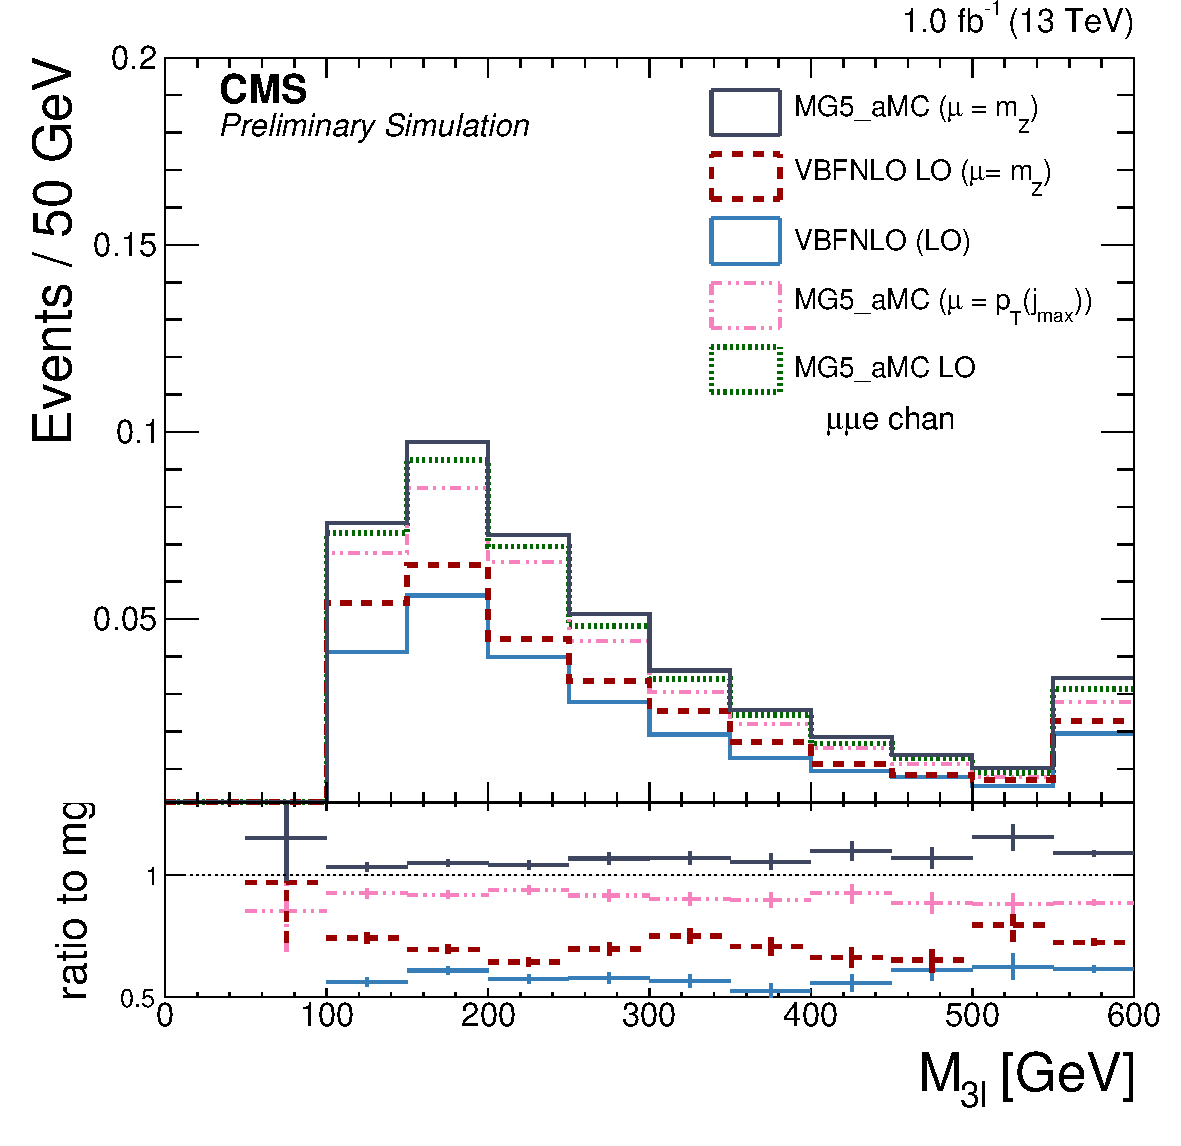
\includegraphics[scale=0.65]{figs/3lmass.pdf}
\caption{A placeholder...}
\label{vbs_fig1}
\end{center}
\end{figure}

\subsection{Conclusions \label{concl}}

We presented a comparison of generators predictions for the

electroweak production of WZ in association with two jets at the LHC, etc... 

Overall these results show that etc...

%\clearpage
\bibliography{vbs_bib}

\end{document}
